\documentclass[12pt]{report}

%Magyar nyelvi támogatás (Babel 3.7 vagy későbbi kell!)
\def\magyarOptions{defaults=hu-min}
%\usepackage[magyar]{babel}

%Az ékezetes betűk használatához:
\usepackage{t1enc}% ékezetes szavak automatikus elválasztásához
\usepackage[utf8x]{inputenc}% ékezetes szavak beviteléhez

% A formai kovetelmenyekben megkövetelt Times betűtípus hasznalata:
\usepackage{times}

%A fejléc láblécek kialakításához:
\usepackage{fancyhdr}

%\usepackage{color}
\usepackage{mathtools}

%%JB
\usepackage{hyperref}
\usepackage{commath}
\usepackage{listings}
\usepackage{xcolor}
\usepackage{graphicx}
\usepackage{subcaption}

%Margók:
\hoffset -1in
\voffset -1in
\oddsidemargin 35mm
\textwidth 150mm
\topmargin 15mm
\headheight 10mm
\headsep 5mm
\textheight 237mm

%%JB 
\linespread{1.3}

\lstdefinestyle{py}{
	xleftmargin=\parindent,
	basicstyle=\linespread{1.0}\footnotesize\ttfamily,
	keywordstyle=\bfseries\color{green!40!black},
	commentstyle=\itshape\color{purple!40!black},
	identifierstyle=\color{blue},
	stringstyle=\color{orange},
	showstringspaces=false,
	frame=single,
	language=Python,
	breaklines=true
}

\lstset{style=py}


\newcommand\todo[1]{\textcolor{red}{#1}}
%\renewcommand\todo[1]{}

\begin{document}

%A FEJEZETEK KEZDŐOLDALAINAK FEJ ES LÁBLÉCE:
%a plain oldalstílust kell átdefiniálni, hogy ott ne legyen fejléc:
\fancypagestyle{plain}{%
	%ez mindent töröl:
	\fancyhf{}
	% a láblécbe jobboldalra kerüljön az oldalszám:
	\fancyfoot[R]{\thepage}
	%elválasztó vonal sem kell:
	\renewcommand{\headrulewidth}{0pt}
}

%A TÖBBI OLDAL FEJ ÉS LÁBLÉCE:
\pagestyle{fancy}
\fancyhf{}
\fancyhead[L]{Implementing a self-scaling convolutional neural network}
\fancyfoot[R]{\thepage}

%A címoldalra se fej- se lábléc nem kell:
\thispagestyle{empty}

\begin{center}
	\vspace*{1cm}
	{\Large\bf University of Szeged}

	\vspace{0.5cm}

	{\Large\bf Department of Informatics}

	\vspace*{3.8cm}


	{\LARGE\bf Implementing a self-scaling\\
		convolutional neural network}


	\vspace*{3.6cm}

	{\Large Bachelor's thesis}

	\vspace*{1.4cm}

	%Értelemszerűen megváltoztatandó:
	{\large

		\begin{center}
			\emph{Author:} \\
			\bf{Jenei Bendegúz}  \\
			\normalfont{student} \\
		\end{center}
		\begin{tabular}{c@{\hspace{4cm}}c}
			\emph{Supervisor:}      & \emph{Supervisor:} \\
			\bf{Varga László Gábor} & \bf{Berend Gábor}  \\
			Senior lecturer         & Senior lecturer           \\
		\end{tabular}

	}

	\vspace*{2.3cm}

	{\Large
		Szeged
		\\
		\vspace{2mm}
		2018
	}
\end{center}

%A tartalomjegyzék:
\begingroup
	\hypersetup{hidelinks}
	\tableofcontents
\endgroup

%A \chapter* parancs nem ad a fejezetnek sorszámot

\chapter*{Tartalmi összefoglaló\\(content summary in Hungarian)}
\addcontentsline{toc}{section}{Tartalmi összefoglaló (content summary in Hungarian)}

\todo{TODO: fordítás}

\chapter*{Task proposal}
%A tartalomjegyzékben mégis szerepeltetni kell, mint szakasz(section) szerepeljen:
\addcontentsline{toc}{section}{Task proposal}

The task of the candidate is to create a framework in which convolutional neural networks can be trained, and the size of these networks are determined automatically. The framework should be able to perform the following:

- Training of a fully convolutional neural network to solve a simple image processing task (e.g., edge detection, automatic thresholding, etc.).

- Determining the size of the ideal neural network. An ideal sized neural network solves the problem with a given layer count and structure with the maximum possible accuracy, while keeping the neuron count minimal among layers.

\chapter*{Content summary}
\addcontentsline{toc}{section}{Content summary}

This thesis falls into the topics of \textit{machine learning} and \textit{digital image processing}. It uses a machine learning technique of training a \textit{fully convolutional network} to perform \textit{edge detection}, which is an image processing task. The focus is not on the training or task itself, instead it is on optimizing the parameters of the network, specifically minimizing the number of layers and the number of masks in the layers, while not sacrificing the accuracy of the network. Similar topics have already been researched before, e.g. in \cite{pruning_web}, \cite{pruning_arxiv} and \cite{understanding}.


The beneficial size for the network is determined by a training process which is capable of saving its state and returning to it later. It is also capable of altering the inner structure of the network temporarily. This is used to test and compare different configurations. The previous techniques are combined with different metrics The training stops when an exiting criterion is met. This results in a network configuration that is regarded as optimal by the current strategy.

Naive and more intelligent strategies were designed, to see which one performs best. A simple strategy would randomly select masks in the network and disable them temporarily. Then it would check if the training can continue without them with around the same accuracy. An intelligent strategy would choose based on various metrics and indicators. There might be use cases for both approaches.

The framework was coded in the \textit{Python} language, utilizing the \textit{tensorflow} library \cite{tensorflow2015-whitepaper}. To aid performance, the training was hardware-accelerated using \textit{NVIDIA} graphics cards with CUDA cores, which are operated by tensorflow through the \textit{CUDA} and \textit{cuDNN} libraries.

\chapter*{Introduction}
\addcontentsline{toc}{section}{Introduction}

In this thesis, a special computer program will be written, which uses a convolutional neural network. It will be special because with the use of a neural network it will be able to dynamically refine how it works to produce a better result, i.e., learn. While classical algorithms are created using human intuition or mathematical formulation, machine learning algorithms are given examples of the right answers it should produce with the given data, allowing it to automatically develop ways of solving a specific problem based on feedback about its own performance.

Integrating the technique of convolution into these networks will make them especially efficient in working with images. This opens up new possibilities, like face recognition, object detection or image reconstruction. Convolutional neural networks are already used for these tasks in areas like security or industrial automation \cite{applications}.

Because images contain large amounts of pixels, convolutional neural networks are computationally demanding, requiring expensive hardware and long training times. A larger neural network has more neurons, so it must perform more operations, making it more demanding than a smaller one. This is why it is important to use a network which has just enough neurons to perform the task accurately, but no more, to avoid unnecessary calculations and computing time.

This thesis attempts to come up with automatic ways of determining the right neuron count and network size for a given problem. This way, no repeated testing and trial-and-error is required, while manually trying different network sizes, because the network will try to find a fitting size for the given problem automatically without requiring human intervention. Existing automatic approaches include exhaustive grid search over a set of parameters. This means repeated training with each combination of the parameters. The method described in this thesis is an alternative way of finding the right parameters. The network is measured and changed during training, as opposed to running it multiple times as in grid search. This is in hope of saving computational resource and reducing training time.

The benefits of using properly sized neural networks include portability and resource efficiency. With less demanding networks, cheaper hardware such as mobile devices will be capable of running convolutional neural networks, making them more widely available. The computational costs can also be reduced, producing results faster and with more modest hardware.
\chapter{Technical overview}
\section{Minimal fully convolutional networks}
The goal of this thesis is to create a framework which is capable of training a deep convolutional neural network for simple two-dimensional image processing tasks and provide ways to make this network as small as possible without sacrificing a considerable amount of its accuracy.

First is a short description of\textit{ artificial neural networks}, or \textit{NNs}, on which convolutional neural networks are based. Artificial neural networks are inspired by the biological neural networks in the brain. An artificial neuron is a simple model of a biological neuron. They can have any number of inputs, originating from other neurons, or directly from the input, sensory organs in case of real neurons. They have exactly one output, which can be connected to an input of another neuron, or channeled to the output. When a neuron gets its inputs, it produces a weighted sum of them, adds a bias, applies a function called activation function. Finally it puts the result on its output.

The \textit{weights} and \textit{bias} within a neuron are its unique parameters that define is characteristics. The activation function is used to introduce some nonlinearity. It is usually a simple linear or exponential function, often cutting negative values, or values falling outside of a range, substituting them with zeros. Neurons are usually grouped into layers, where they do not connect to each other, only to other immediate (also called hidden), input or output layers. When an immediate layer passes its outputs to another immediate layer, we are speaking of a \textit{deep neural network (DNN)}.

To mimic the learning capability of intelligent species, artificial neural networks perform feedback based learning by altering the unique weights and biasing of the neurons. A loss function is defined for every neural network, which produces a value which is proportional to how well the network performs. For example, in case of classification, it is proportional to the confidence of the network about an incorrect class, where bigger values mean poorer performances. Using this value, the weight and bias parameters of the neurons are altered based on their contribution to the error or score. This improves score value and thus the performance of the network. This process is called \textit{error back-propagation} or \textit{training}.

The size of a deep neural network is defined by two parameters: \textit{number of layers}, and \textit{number of neurons} in each layer, which can vary between layers. These parameters must be specified when building a neural network for training. This thesis will try to provide automatic strategies to come up with beneficial values for these two parameters, as opposed to defining them with trial \& error, repeated manual testing, or based on experience.

\textit{Fully convolutional networks}, or \textit{FCNs} are derived from convolutional neural networks. Convolutional neural networks were first used for classification \cite{applications}. Their first layers were convolutional layers performing feature extraction. The last layers were fully connected layers of neurons, performing the classification or regression using the extracted features. FCNs let the images be images, making a network which gets images as input and throws back images as output. This makes them able to mark interesting parts of an image, or perform numerous other image processing tasks.

The network needs a task which gets an image as input and gives back another image. This leads us to a simple non-trivial two-dimensional image processing task that can be learned in feasible times. Meanwhile the quality of the edge maps are somewhat subjective, each method having its strong and weak areas. Below are the two chosen image processing tasks. Other, very different tasks could have been chosen, which is a possible direction for further experimentation.
\section{Edge detection}
An \textit{edge} in image processing is a sudden change in pixel intensity within an image. This is common on the edges of objects, or at the intersection of different colors in a pattern. There are no criteria for the actual required value of the intensity-change per pixel, so there is no single right solution for edge detection. There are multiple techniques available for detecting edges, each having its own strengths and weaknesses.

There are two classes of edge detection, based on their output format: \textit{continuous} and \textit{discrete}. \textit{Continuous} detectors produce an image of the same dimensions as the source image, where a pixels intensity value corresponds to how strong of an edge is present at that position in the original image. \textit{Discrete} detection uses boolean values to tell if an edge is present or not. Continuous detections can be converted to discrete by thresholding, or using adaptive thresholding on parts of a continuous edge map.

Edges can occur in any direction on an image. The detectors often use derivatives and gradients to determine the sudden drops and rises in intensity, among both axes. Since most detectors use multiple steps until they produce the final edge map, it could make sense to use a deep, multi-layered network to see if a layer could more-or-less represent a step in the process. \textit{Convolving} an image with an appropriate mask is also used in edge detection. A \textit{convolutional network} is capable of learning and applying combinations of masks automatically.
\subsection{Conventional algorithmic edge detectors}
The following two edge detectors are important, as they are widely used algorithms, their output will serve as examples of edge maps.

The \textit{Sobel–Feldman operator}, or \textit{Sobel filter} \cite{sobel} consists of two discrete matrices to be convolved with the source image. This will result in two edge map images, or gradients, one for the horizontal and one for the vertical axis. Then the two matrices can be combined by calculating the geometric mean pixel-wise. The result is a continuous edge map.

The \textit{Canny edge detector} \cite{canny} is a more complex one, consisting of five steps, including filtering, gradient computing, non-maximal edge suppression, double thresholding, and hysteresis to suppress weak edges. The first two steps can be carried out with convolutional masks, while the latter ones are algorithms. The Canny edge detector as opposed to the Sobel operator will result in a discrete edge map.
\subsection{Using the detectors}
Sobel edge detection and the first two steps of Canny edge detection can be carried out with convolutions, so they can theoretically be learned by the network. The latter steps of Canny edge detection are algorithmic, thus they cannot be directly learned.
This will force the network to find its way around the problem, come up with alternative methods using convolutional masks in order to optimize the objective function.

The network will be trained with raw images, and images ran trough the Canny and Sobel edge detectors. The objective of the network will be to mimic the outcome of the detectors. First, we will train with the Sobel detector. This should be the easier task for the network, since everything can be done with convolutions with the correct masks. Then, we will use the Canny detector, which is considered a harder task due to the multiple steps including different algorithms.

The input will be a raw image encoded and compressed in png format, this is what the network will get to work on, and the sample output will be an edge map, made with either the Sobel operator or the Canny operator. The objective function will ensure that the actual output is as close to the sample output as possible, by producing a high penalty if they differ.
\section{Tools}
There are a variety of machine learning toolkits and frameworks to choose from. Some of the major criteria is the ability to freely customize as much aspects as possible, while also being able to quickly produce a working implementation for fast experimentation. These seemingly conflicting points ask for a framework which is not too high or too low-level. The physical tools, the hardware, must be chosen as well, based heavily on availability and possessions.
\subsection{Software}
\textit{Python} is an open source interpreted programming language, which is widely used in machine learning, or for writing simple tools, thanks to its fluent syntax. Most major machine learning frameworks (tensorflow, Caffe, Caffe2, CNTK and so on) support Python, often as the main language. It is easy and fast to implement and test a new idea, due to it being a high level language, but the performance cost of it is negligible. The most demanding part of machine learning is not the network building part, which is the part Python is used for. It is the training itself, repeatedly evaluating the network, calculating the error and propagating it backwards. This part is usually made to be hardware accelerated by most frameworks.

\textit{Tensorflow}, being developed by Google, is a framework for making and using computational graph, supporting the creation of deep neural networks. It is used for both research and as a backend for PC and mobile applications, or the core on which higher level frameworks build on. Tensorflow is based on Python, and it has limited support for C++. There are two ways to make graphs with the toolkit: high level and low level. In the higher level, there are several predefined layers available, these can be parametrized stacked on top of each other to produce a graph. The most common machine learning network layouts are supported by this method. In the lower level, exact operations (addition, convolution, transposing, etc.) and the flow of the data must be coded. This method is used to develop tools for higher level tensorflow, and for research, because of the freedom of configuration it provides. While being lower level, there are still numerous tools and helper functions available, even image file decoders and preprocessors for example. Another strength of tensorflow is hardware acceleration. With a supported NVIDIA graphics card, computational graphs can be executed in GPU accelerated mode, which is often faster than CPU mode by several magnitudes. The version used was 1.6, the latest stable release at the time of coding.

\textit{CUDA} by \textit{NVIDIA} is required to utilize the computing capacity of a supported GPU, and run tensorflow in GPU accelerated mode. CUDA is crossplatform, available for Windows, macOS and Linux, and it is downloadable freely.

\label{cudnn}
\textit{cuDNN}, the \textit{CUDA Deep Neural Network} library provides GPU-accelerated routines for common machine learning tasks. It is also available for free, but a registration is required, specifying the plan of usage and associated institutes as well. Tensorflow, when used in GPU mode, relies on this library. One negative effect of this is the non-deterministic nature of some routines, and tensorflow provides no way around it. This way, getting the same exact outcome in two different runs is not possible. Using seeding to achieve this would produce more comparable result, without this technique more testing is required. The exact operation which is affected will be described at section \ref{train}.
\subsection{Hardware}
Initially a relatively low performance notebook was used to perform all the training. The main benefit of using this notebook was its built-in dedicated GPU, the NVIDIA GeForce 840M. It has 384 CUDA cores with compute capability version 5.0, which means it is able to run tensorflow in GPU-mode. Tensorflow demands compute capability to be 3.0 or higher to run in GPU-mode, 3.0 and 3.5 are common among machine learning toolkits. The notebook had 4GB RAM, and 2GB VRAM.

Later, several tests were ran remotely at a higher performance desktop computer, while the notebook was used to develop the models and check if they work as intended. These runs were often longer than a week, depending on the sample size. This PC was an Intel Core i7-6700 with 16GB RAM, and it had an NVIDIA Tesla K40 GPU with 12GB VRAM and 2880 CUDA cores.
\chapter{Implementation}
\section{Preparing the input images}
A large and openly available set of images were needed as input for the training. The Visual Object Classes Challenge 2012 (VOC2012) dataset \cite{pascal-voc-2012} was chosen for this purpose. The VOC dataset contains colored pictures of 20 classes in different settings. Classes include aeroplane, people, bicycle, horse and so on. These are fine for simple image processing tasks, there are a wide variety of objects in various distances and quantities. The classes are not needed for us, since we are outputting an image the same dimensions as the input, instead of performing classification. Without the classes, the expected output for training had to be generated from the input images, this was done with matlab scripts and built-in image processing functions.

The images and edge maps are fed to the network during training. The images must be preprocessed to be in an efficient format for training. The goal is to have matrices which can run trough the FCN and produce an output. First the center of the images are cropped, because the input pipeline uses a fixed structure, and the dataset has pictures of varying size. The size of the area to be cropped is $256\times256$, meaning this is the dimension of the images the network will work on. Then, the images are decoded to pure matrices containing floating point values. After this we will have three dimensional images due to the RGB color palette, this is reduced to two dimensions by converting the image matrices to grayscale. This way the color information is lost. Effectively using the color channels to improve edge detection precision is a different area of research, which is not discussed here. Finally, a number of images are batched together to enable bulk processing of inputs, leaving us with an input shape of $ batch\ size\times image\ height\times image\ width $. With the batch size set to $3$, the actual shape is $ 3\times 256\times 256 $.
\section{Network structure}
This section explains the parameters of the FCN, including the types and sizes of the layers, the objective functions and the metrics used.

In tensorflow, the network we build is a computational graph. The vertices are operations or placeholders while the edges are the data flowing in one direction, joined to one or more vertices. The edges are also called tensors, they can be simple numbers or multidimensional matrices, images or groups of images for example.
When defining multi-dimensional variables, the tensorflow-recommended \textit{NHWC} format is used where possible: $ N:batch,\ H:height,\ W:width,\ C:channels. $ This forces some consistency into the code and structure. Most built-in tensorflow functions expect this format, so no reshaping is required, and there is also a benefit in performance, since this is the optimal format for CUDA operations as well.
 
Our FCN is made up by three layers, the first layer gets the reprocessed image from the previous section, while the third layer produces the output image. The layers are convolutional with an added bias, initialized randomly with a predefined distribution.

Each \textit{convolutional layer} has its own set of five masks sized $5\times5$. Strides and dilations are set to one in all dimensions, this means no pixels are skipped when convolving the whole image. A 5x5 mask allows for more complexity than a $3\times3$ mask, while being able to produce the same results if the weights on the edges are small enough. After a convolution is performed with a mask, a scalar bias is added elementwise to the resulting pixels.

\textit{Truncated normal initialization} \cite{trunc} is used before the first training. The values are derived from a general normal distribution parametrized by a given mean and deviation. Truncated means that values with more than two standard deviations distance from the mean are redrawn, this will chop off the edges of the histogram, producing a more even distribution with fewer outliers. The mean and standard derivation were set to $0.0$ and $ 5\times10^{-2} $.

The \textit{activation function} is \textit{ReLu} (rectified linear unit) \cite{relu} across the whole network. ReLu is a simple linear rectifier, returning zero for negative values and the original value otherwise. It is a convenient choice because due to its linearity it does not deform the images. It is also fast to compute and widely used for convolutional networks. Since ReLu has no upper limit, the final output must be scaled down and rounded to fit an image format standard, usually $ \left[0;255\right] $ or $ \left[0;1\right] $. First we shift the range if needed to get positive values, then scale it to $ \left[0;255\right] $. Finally we convert the image to \textit{png} format using rounded and unsigned 8-bit integers.
\subsection{The objective function and output}
The objective function must return a single number which the optimizer will try to minimize or maximize. In our case this will be minimization, the tensorflow optimizers default to this. The framework being made for this thesis has some options to specify the objective function before training, so testing different losses can be automatized. A few fitting objective functions were tested, and the ones which produce high accuracy the faster were kept. The error-calculating operation gets the output and expected output as inputs, its result is used by the training operator, and the error can be written to the console for information.

Training with the Sobel edge map dataset, we have a continuous output and a set of continuous example images, so the objective function must take two batches of continuous matrices to calculate the error. L1 and L2 losses work with the difference of the matrices. L1 loss or mean absolute error (MAE) calculates the mean of the absolute difference matrix, L2 loss or mean squared error (MSE) calculates the average of the squared values of the difference matrix:
\begin{equation*}
MAE = \frac{1}{N}\frac{1}{H\times W}\sum_{y=1}^{H}\sum_{x=1}^{W}\abs{O_{n,y,x}-\hat{O}_{n,y,x}}\ \ ,
\end{equation*}
\begin{equation*}
MSE = \frac{1}{N}\frac{1}{H\times W}\sum_{y=1}^{H}\sum_{x=1}^{W}\left(O_{n,y,x}-\hat{O}_{n,y,x}\right)^{2}\ \ ,
\end{equation*}
where $N$ is the batch size ($3$), $H$ and $W$ are the image dimensions ($128\times128$), $O$ is the actual output of the network and $\hat{O}$ is the expected output. These losses are common with regression. The reason behind squaring the values is to achieve shorter training times, because bigger errors are penalized exponentially more.

Training with the Canny edge map dataset, we have a continuous output, but a discrete expected output, matrices that containing either ones or zeros. L1 and L2 loss can be also used here. To account for false positives and negatives (\textit{FP} and \textit{FN}), and true positives and negatives (\textit{TP} and \textit{TN}), a modification of the confusion metric F1 score is also used. F1 score originally operates on discrete values, and here only the expected output is discrete, this will not be a true F1 score, but it will follow the same principles. The result must also be negated (subtracted from one) to get a loss, which is inversely proportional to the accuracy. The definition of F1 score is
\begin{equation*}
	\frac{2TP}{2TP + FP + FN}\ \ ,
\end{equation*}
where we can replace the addition of both types of negatives with the error value to simplify the formula to
\begin{equation*}
	\frac{2TP}{2TP + E}\ \ ,
\end{equation*}
where $ E $ is the error of the current example. The negated version to produce a loss instead of a score becomes
\begin{equation*}
	1 - \frac{2TP}{2TP + E} = \frac{2TP + E - 2TP}{2TP + E} = \frac{E}{2TP + E}\ \ .
\end{equation*}
Defining F1 score and loss for the model in tensorflow:
\begin{center}
	\begin{minipage}{0.95\textwidth}
		\begin{lstlisting}[title=fcn\_model.py]
...
def f1_loss(output_image, output_image_train):
	difference = tf.reduce_sum(tf.abs(output_image - output_image_train), [1,2,3])
	TP = tf.reduce_sum(output_image * output_image_train, [1,2,3])
	f1 = tf.reduce_mean(difference / (difference + 2 * TP))

	return f1

def f1_score(output_image, output_image_train):
	difference = tf.reduce_sum(tf.abs(output_image - output_image_train), [1,2,3])
	TP = tf.reduce_sum(output_image * output_image_train, [1,2,3])
	f1 = tf.reduce_mean(2 * TP / (2 * TP + difference))

	return f1
...
		\end{lstlisting}
	\end{minipage}
\end{center}
And outside of tensorflow with NumPy as a metric to use during validation:
\begin{center}
	\begin{minipage}{0.95\textwidth}
		\begin{lstlisting}[title=metrics.py]
...
def f1_score(output_image, output_image_train):
	if output_image.shape != output_image_train.shape:
		print('f1_score: image sizes not equal, exiting')
		import sys
		sys.exit()

	difference = np.sum(np.abs(output_image - output_image_train))
	TP = np.sum(output_image * output_image_train)
	f1 = np.mean(2 * TP / (2 * TP + difference), dtype=np.float64)

	return f1
...
		\end{lstlisting}
	\end{minipage}
\end{center}

\subsection{Training and error back-propagation} \label{train}
The training operation is joined last after the layers, right after the operation that calculates the error from the output, but it reads and manipulates almost the whole graph. It computes the gradients of all the operations in the graph, and then changes the trainable variables weighted by their contribution to the error.

One of the tensorflow built-in optimizers, \textit{Adam} \cite{adam} is used. It features momentum-based dynamic learning rate, which promises improved convergence time over SGD \cite{sgd}, on which it is based. SGD is short for \textit{stochastic gradient descent}. It is a gradient descent variant which only uses a random subset of the training examples to approximate the gradients in each training step. This makes the calculations cheaper and shortens the training steps. The approximation becomes more accurate as we increase the size of this subset. There is a variety of SGD modifications developed that add a dynamic and adaptive behavior, Adam is one of them. Adam has two built-in running variables, which change over time, resulting in smaller weight updates as time progresses during training. Because of cuDNN, as mentioned in section \ref{cudnn}, Adam is slightly non-deterministic even when used with the same parameters and random-seed. The cause of the non-reproducible results was the implementation of some reductions using asynchronous CUDA atomic operations. This has been resolved in later tensorflow versions, but was still present in the used version (1.6). See \cite{nondet1} and \cite{nondet2}.

\textit{Training} and \textit{evaluation} steps are alternating during a training session. Training steps take up the majority of the time, while evaluation or validation steps are around ten or more times less frequent during a run. Both steps iterate on their own separate set of data. These two sets are sometimes created by splitting one large dataset by a ratio favoring the training split. For both the Sobel and Canny tasks, we use 20000 images for training and roughly 14000 images for evaluation.

A \textit{step} during training consist of producing one error value from the input and output, and performing back-propagation once to modify the trainable variables, or weights. This does not mean that one step takes exactly one image, since batching is used, so one step deals with a batch of images. The processing time a resources needed for a step depends on the batch size.

With each \textit{training step}, the error is calculated and back-propagation is performed. An \textit{evaluation step} stops right before calculating the error, and only produces the output image, so no back-propagation is happening here. This leaves the network untouched. The purpose of this is to measure the accuracy on the evaluation set, which is invisible to the network during training. Evaluation is also used to produce more and prettier metrics for the human observer. Evaluation runs less rarely than training, so heavier computation on metrics are possible without slowing down the training process.
\section{Minimization}
Minimization refers to reduction in the size of the FCN. This section is about the methods and tricks which make it possible to change the network during training, step back to an earlier state and compare states. This way determining the minimal size for the FCN can be automatized.

After each change in the network, including all of the methods described below, additional steps are necessary. The Adam \cite{adam} optimizer uses parameters that change over time. It has accumulators, and also a variable storing the step number, which represents the passing of time. The greater these variables, the less likely that the trainable variables receive big updates. When they are reset, we are giving each network configuration equal chances. We reset these parameters every time the network is altered or reverted to give the modified network a fresh start in training. \todo{TODO: kódrészlet} These variables are not easily accessible, there are no helper methods provided. We must manually reach into the graph and reinitialize them.
\subsubsection{Neglecting neurons}
To simulate a graph with fewer masks, or ,,neurons'', the masks can be disabled any time during training. Masks are contained in multidimensional matrices, one mask for each edge or input that the vertex or operation receives. Since the structure of the cannot be modified, we include switches into it, which tell exactly which neurons are disabled. The disabled masks always produce an output of zeros, whatever their input might be. Disabling masks provides no performance advantage, since they are still in the graph, taking up memory, but if we find that the results are still accurate with a few masks disabled, it means that the problem is solvable with fewer masks.
\subsubsection{Freezing neurons}
Freezing a mask means that the frozen mask will not receive updates via back-propagation, but will still produce an output. This is implemented similarly to disabled masks, providing switches that toggle between giving the mask zero-gradient, or retaining its value.
\subsubsection{Reinitializing neurons}
Reinitializing the masks instead of giving them zero values is also considered. The reason is that before the first run, the masks were given initial values based on normal distribution, instead of zeros, which should provide accelerated learning speed.
\subsubsection{Stepping back}
After a couple of training steps, we evaluate the accuracy, and save a snapshot of the graph to disk. This allows for resumed training later. This way we can compare thecurrent metric with earlier ones, and revert to them if we wish, for example when the accuracy had decreased since. Tensorflow provides functions to save and resume the graph structure, called meta-graph, and a checkpoint, which will store the current values of all free variables.

This is not hassle free. Tensorflow stores the absolute paths of the meta-graph and checkpoints into a plain text file name 'checkpoint'. In order to be able to move a saved model around, this file is altered by the training script to reflect the actual folders when resuming the network.

Another problem is that by default, tensorflow automatically saves every variable it can find, and constant values are incorporated into the graph. The graph cannot be touched after it was reloaded, so everything what needs changing later must be a variable. In order to prevent the saver from incorporating the input file list into te graph, and bloating it with thousands of file paths on each resume, the input pipeline must be set up separately from the rest of the graph, which needs to be feedable with the filenames. This way the saved model can be resumed and initialized with a new set of inputs, without storing them in the graph.
\subsection{Testing the worth of a neuron}
There are a few ways to utilize freezing and disabling to determine how much a single mask contributes to the overall accuracy, and see how the network performs without it.
\subsubsection{One disabled}One selected mask is disabled. This is useful to test the accuracy without that mask, and also observe what the optimizer will train this mask the next time.
\subsubsection{One disabled and frozen}The same as the above, plus the mask is frozen as well. This would provide insight to how the rest of the network will change when this mask is removed, whether it will learn to take its role, or remain unchanged.
\subsubsection{One disabled, others frozen}The rest of the net is frozen, this will prevent the net from compensating the absence of the mask, but lets the mask relearn.
\subsection{The minimization process}
This process encapsulates multiple training sessions, and uses the tools and methods described above between them in hope of determining a minimal configuration.

First, a training session is invoked to produce a working network that is close to convergence and is capable of inference. This is longer than the later sessions, $10000$ steps in most runs. We are ready to stop the training when error stagnates. The network is then evaluated and saved to disk. Then one or more masks are \textit{selected} and altered. Altering includes freezing and disabling masks, and there are multiple strategies for \textit{selection}, they are described below. After this, another training session and evaluation is performed with the altered network. This is shorter because the network is already semi-converged, $2000$ steps exactly. The results of the new evaluation and the old one are compared, and if the new one is weaker, the old network is reloaded from disk. The strength of the new network compared to the old one is determined by a threshold over the ratio of their evaluation performance. Evaluation performance is measured by computing the mean F1 score over the evaluation dataset. Multiple thresholds were tested: $ 85\%,\ 90\%,\ 95\%,\ 98\%$ and $100\%$. Then comes another selection, which makes sure to select different masks if the network was restored. The sequence of training, evaluation, comparison and \textit{selection} is repeated until the stopping criteria are met. We are left with the final network, and a one-hot matrix which describes which masks ca be removed to get the minimal structure.
\subsection{Selection}
Masks have to be selected, for freezing or disabling, the choice should reflect the contribution of the selected mask to the overall performance, or in other words, the least important mask should be the one that gets selected, so the network could possibly perform with one less mask.
\subsubsection{Cosine-similarity}Cosine similarity  tries to represent how similar two n-dimensional vectors are. A mask is a set of two-dimensional matrices plus scalar biases, so they are reshaped to a vector format, with the bias appended to the end of the vector. Then all the vectors are compared to each other using cosine similarity, and the end result is stored in a matrix, where the element at indices $i$ and $j$ represents the cosine similarity between the the mask in place $i$ and the mask in place $j$. These values have a range of $\left[-1;1\right] $, where $1$ represent the greatest similarity (vectors facing the same direction), while negative numbers represent opposites (vectors facing the opposite direction). This is done for each layer, producing a matrix for each layer.

Using the matrices, selection could be done by selecting the mask which is most similar to the others, so it has the highest average similarity, or the one which has the maximal single similarity. These strategies hypothesize that a mask that is really similar to other masks is redundant, while unique masks play a key role in the inference. Absolute value could be used on the similarity values, since negative similarity could still mean similarity in the FCN.

An extension to this method is to use the second, or n-th maximal mask after the previous one failed and produced a significant decrease in performance.
\subsubsection{Naive selection strategies}
\paragraph{Sequential}This method simply goes through every mask in a sequential order. This is mostly useful for comparison for smarter strategies.
\paragraph{Random}
Randomly picks a mask. Also useful for comparison, but it also could be a viable strategy.
\chapter{Metrics}
In addition to the objective function, or error, which is a metric itself the following metrics were used to judge the performance. These were used in the validation steps, or separately from training to benchmark the network.
\section{Universal Image Quality Index}This metric is used to rank the similarity of two images. It is produced from three components, measuring the correlation, luminance difference and contrast difference between the two input images. It works by splitting the images into sections with a chosen size, and calculating the metric on those. We calculate an average of these to get a single value. When used alongside the simpler MAE and F1 score, this could provide an alternative metric and view on accuracy. A matlab implementation was provided by the authors, which was then converted to python so it can be integrated into the training process.
\section{Visualization}Visual representation of the masks and snapshots of the inputs at each stage as they travel through the network are printed as image files to disk. This way the inner workings of the net are somewhat observable. Masks and images apart from the final output can contain negative values. To illustrate the whole range, negative values are visualized red, positive values are visualized green and color intensity represents absolute value. Examples of these visualizations are shown below. Note that some of the top masks resemble edge detector operators (see \cite{sobel}), and the output of the very first mask resembles a diagonal edge map.
\begin{figure}[h!]
	\centering
	\begin{subfigure}[b]{0.4\linewidth}
		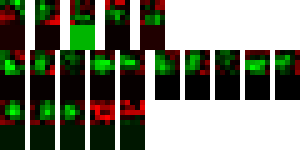
\includegraphics[width=\linewidth]{images/masks_before.png}
		\caption{Masks after a few steps...}
	\end{subfigure}
	\begin{subfigure}[b]{0.4\linewidth}
		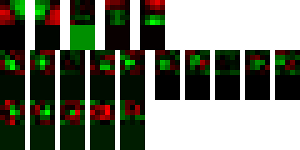
\includegraphics[width=\linewidth]{images/masks_after.png}
		\caption{...and after convergence}
	\end{subfigure}
	\caption{Mask visualizations, rows on the picture correspond to layers in the network. The first row represents the masks in the first layer. Three groups of five masks from the second layer are omitted.}
\end{figure}
\begin{figure}
	\centering
	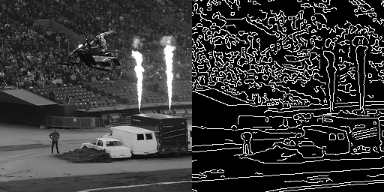
\includegraphics{images/out1.png}
	\caption{An input and ground truth image}
	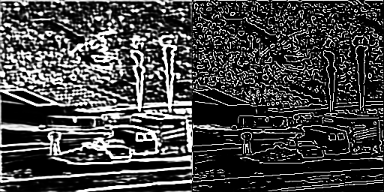
\includegraphics{images/out2.png}
	\caption{Output after a few iterations and after convergence}
\end{figure}
\begin{figure}
	\centering
	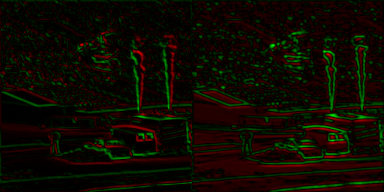
\includegraphics{images/layer1.png}
	\caption{The output of the first mask in the first layer and the final output before activation, both after a few steps...}
	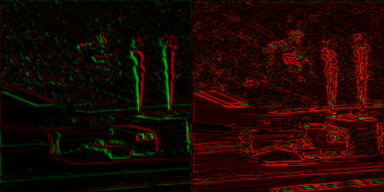
\includegraphics{images/layer2.png}
	\caption{...and the same after convergence}
\end{figure}

\chapter{Results}
\section{Run 1}
freezing
\section{Run 2}
correlations
\section{Run 3}
final
\chapter{Conclusion}
\chapter{Appendix}
\chapter*{Statement}
%Egy üres sort adunk a tartalomjegyzékhez:
\addtocontents{toc}{\ }
\addcontentsline{toc}{section}{Statement}
%\hspace{\parindent}

% A nyilatkozat szövege más titkos és nem titkos dolgozatok esetében.
% Csak az egyik tipusú myilatokzatnak kell a dolgozatban szerepelni
% A ponok helyére az adatok értelemszerűen behelyettesídendők es
% a szakdolgozat /diplomamunka szo megfeleloen kivalasztando.

%A nyilatkozat szövege TITKOSNAK NEM MINŐSÍTETT dolgozatban a következő:
%A pontokkal jelölt szövegrészek értelemszerűen a szövegszerkesztőben és
%nem kézzel helyettesítendők:

\noindent
Alulírott \makebox[4cm]{\dotfill} szakos hallgató, kijelentem, hogy a dolgozatomat a Szegedi Tudományegyetem, Informatikai Intézet \makebox[4cm]{\dotfill} Tanszékén készítettem, \makebox[4cm]{\dotfill} diploma megszerzése érdekében.

Kijelentem, hogy a dolgozatot más szakon korábban nem védtem meg, saját munkám eredménye, és csak a hivatkozott forrásokat (szakirodalom, eszközök, stb.) használtam fel.

Tudomásul veszem, hogy szakdolgozatomat / diplomamunkámat a Szegedi Tudományegyetem Informatikai Intézet könyvtárában, a helyben olvasható könyvek között helyezik el.

\vspace*{2cm}

\begin{tabular}{lc}
	Szeged, \today\
	\hspace{2cm} & \makebox[6cm]{\dotfill} \\
	& aláírás \\
\end{tabular}

\vspace*{4cm}

\chapter*{Acknowledgments}
\addcontentsline{toc}{section}{Acknowledgments}

Ezúton szeretnék köszönetet mondani \textit{X. Y-nak} ezért és ezért \ldots

%% Az itrodalomjegyzek keszitheto a BibTeX segedprogrammal:
\bibliography{references} 
\bibliographystyle{unsrt}

\end{document}